\documentclass[twoside]{article}
\usepackage{../estilo-ejercicios}
\usepackage{wasysym}
\usetikzlibrary{automata,positioning}
%--------------------------------------------------------
\begin{document}

\title{Ciencias de la Computación}

\author{Javier Aguilar Martín}
\maketitle

\begin{ejercicio}{1}
Sea $M$ la máquina de Turing de lenguaje $Σ = \{1\}$ y tabla de transiciones:
\begin{align*}
	(q_1,B,R,q_2)\\
	(q_2,1,R,q_3)\\
	(q_3,B,R,q_4)\\
	(q_4,1,B,q_1)\\
	(q_4,B,R,q_4)
\end{align*}
Supongamos que $q_1$ es el estado inicial de $M$. Para cada $x \in \N$ sea $g(x)$ el número de $1$'s que quedan en la cinta de $M$ tras dentenerse la computación de $M$ iniciada sobre una cadena de $x$ $1$'s con la cabeza lectora situada a la izquierda del primer $1$. ¿Cual es la función $g : \N \dashrightarrow \N$ calculada por $M$ de este modo?
\end{ejercicio}

\begin{ejercicio}{2}
Para cada una de las funciones siguientes, escríbase un programa de Post-Turing que la calcule ($x$ e $y$ denotan palabras sobre el alfabeto $Σ = \{a,b\})$:
\begin{enumerate}
	\item $f_1(x,y)=xy$.
	\item $f_2(x,y)=yx$.
	\item $f_3(x) = x^R$, siendo $x^R$ la palabra cuyos símbolos son los de $x$ en orden inverso.
	\item $f_4(x) = \begin{cases}
		a &\text{ si }|x|\text{ es par}\\
		b &\text{ si }|x|\text{ es impar}
	\end{cases}$
\end{enumerate}
\end{ejercicio}

\begin{ejercicio}{3}
Para cada una de las funciones siguientes, proporcionar una máuina de Turing que la calcule ($x$ e $y$ denotan palabras sobre el alfabeto $Σ = \{a,b\})$:
\begin{enumerate}
	\item $f_1(x)=abx$.
	\item $f_2(x)=axb$.
	\item $f_3(x,y)=xy$.
	\item $f_4(x,y)=yx$.
	\item $f_5(x)=x^R$, siendo $x^R$ la palabra cuyos símbolos son los de $x$ en orden inverso.
\end{enumerate}
\end{ejercicio}
\begin{sol}\mbox{}
\begin{enumerate}
	\item \hfill

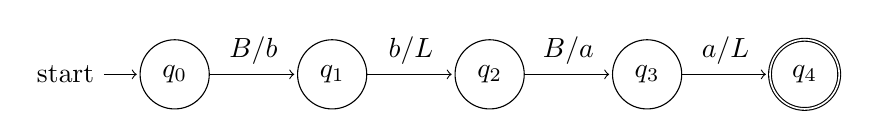
\begin{tikzpicture}[shorten >=1pt,node distance=2cm,on grid,auto]
   \node[state,initial] (0) {$q_0$};
   \node[state] (1) [right=of 0] {$q_1$};
   \node[state] (2) [right=of 1] {$q_2$};
   \node[state] (3) [right=of 2] {$q_3$};
   \node[state,accepting] (4) [right=of 3] {$q_4$};
   \path[->]
    (0) edge                    node {$B/b$} (1)
    (1) edge                    node {$b/L$} (2)
    (2) edge                    node {$B/a$} (3)
    (3) edge                    node {$a/L$} (4)
    ;
\end{tikzpicture}

	\item \hfill

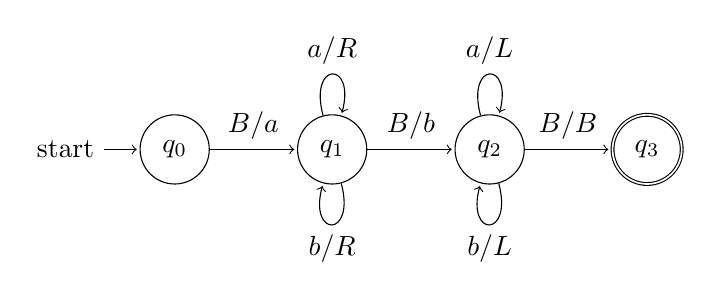
\begin{tikzpicture}[shorten >=1pt,node distance=2cm,on grid,auto]
   \node[state,initial] (0) {$q_0$};
   \node[state] (1) [right=of 0] {$q_1$};
   \node[state] (2) [right=of 1] {$q_2$};
   \node[state,accepting] (3) [right=of 2] {$q_3$};
   \path[->]
    (0) edge                    node {$B/a$} (1)
    (1) edge  [loop above]      node {$a/R$} (1)
    (1) edge  [loop below]      node {$b/R$} (1)
    (1) edge                    node {$B/b$} (2)
    (2) edge  [loop above]      node {$a/L$} (2)
    (2) edge  [loop below]      node {$b/L$} (2)
    (2) edge                    node {$B/B$} (3)
    ;
\end{tikzpicture}

	\item \hfill

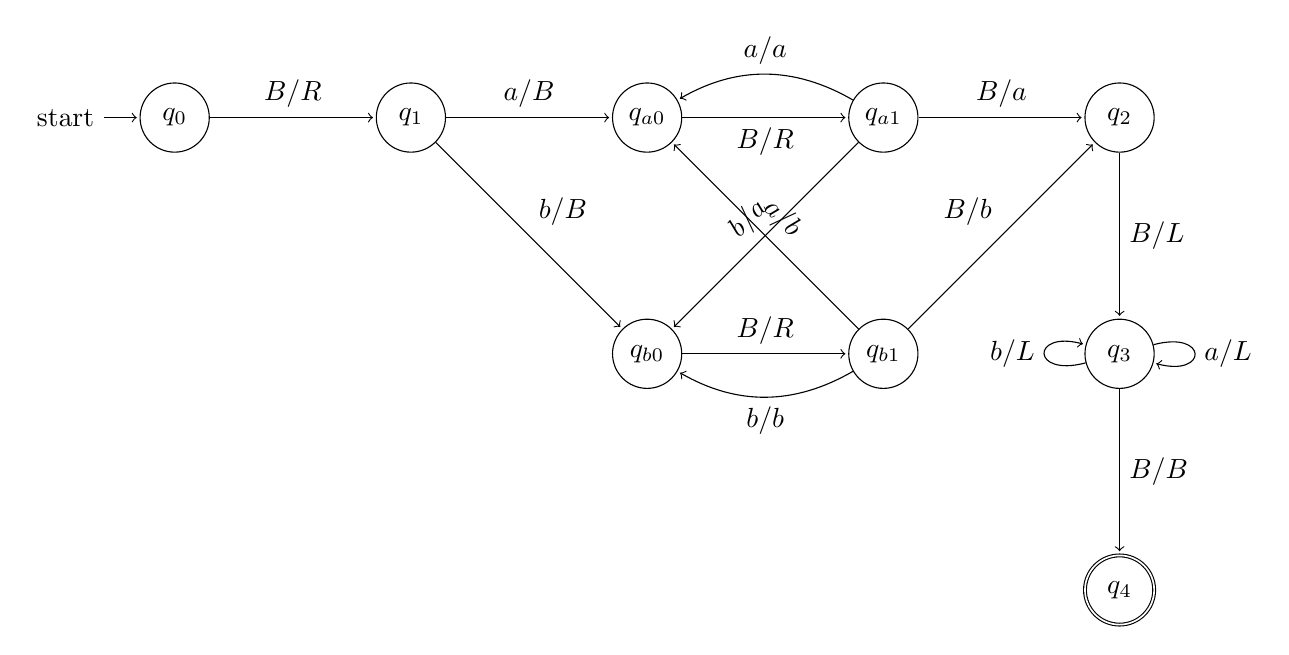
\begin{tikzpicture}[shorten >=1pt,node distance=3cm,on grid,auto]
   \node[state,initial] (0) {$q_0$};
   \node[state] (1) [right=of 0] {$q_1$};
   \node[state] (a0) [right=of 1] {$q_{a0}$};
   \node[state] (a1) [right=of a0] {$q_{a1}$};
   \node[state] (2)  [right=of a1] {$q_2$};
   \node[state] (b0) [below=of a0] {$q_{b0}$};
   \node[state] (b1) [right=of b0] {$q_{b1}$};
   \node[state] (3)  [below=of 2]  {$q_3$};
   \node[state,accepting] (4)  [below=of 3]  {$q_4$};
   \path[->]
    (0) edge                    node {$B/R$} (1)
    (1) edge                    node {$a/B$} (a0)
    (1) edge                    node {$b/B$} (b0)
    (a0) edge                   node [below] {$B/R$} (a1)
    (a1) edge                   node {$B/a$} (2)
         edge  [bend right]     node [above] {$a/a$} (a0)
         edge                   node [sloped] {$b/a$} (b0)
    (b0) edge                   node {$B/R$} (b1)
    (b1) edge                   node {$B/b$} (2)
         edge  [bend left]      node {$b/b$} (b0)
         edge                   node [sloped] {$a/b$} (a0)
    (2)  edge                   node {$B/L$} (3)
    (3)  edge  [loop right]     node {$a/L$} (3)
         edge  [loop left]      node {$b/L$}
    (3)  edge                   node {$B/B$} (4)
    ;
\end{tikzpicture}

\item \hfill

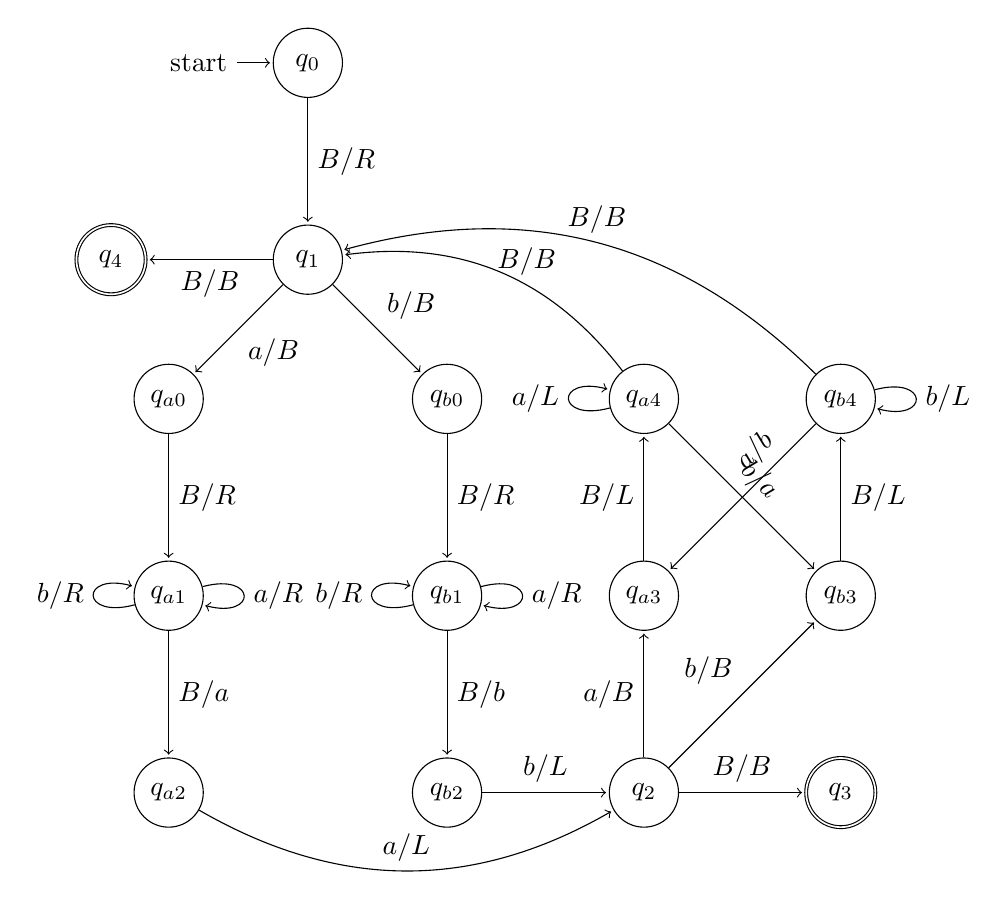
\begin{tikzpicture}[shorten >=1pt,node distance=2.5cm,on grid,auto]
   \node[state,initial] (0) {$q_0$};
   \node[state] (1) [below=of 0] {$q_1$};
   \node[state] (a0) [below left=of 1] {$q_{a0}$};
   \node[state] (a1) [below=of a0] {$q_{a1}$};
   \node[state] (a2) [below=of a1] {$q_{a2}$};
   \node[state] (b0) [below right=of 1] {$q_{b0}$};
   \node[state] (b1) [below=of b0] {$q_{b1}$};
   \node[state] (b2) [below=of b1] {$q_{b2}$};
   \node[state] (2) [right=of b2] {$q_2$};
   \node[state,accepting] (3) [right=of 2] {$q_3$};
   \node[state,accepting] (4) [left=of 1] {$q_4$};
   \node[state] (a3) [above=of 2] {$q_{a3}$};
   \node[state] (a4) [above=of a3] {$q_{a4}$};
   \node[state] (b3) [right=of a3] {$q_{b3}$};
   \node[state] (b4) [above=of b3] {$q_{b4}$};
   \path[->]
    (0) edge                    node {$B/R$} (1)
    (1) edge                    node {$a/B$} (a0)
    (1) edge                    node {$b/B$} (b0)
    (1) edge                    node {$B/B$} (4)
    (a0) edge                   node {$B/R$} (a1)
    (a1) edge [loop right]      node {$a/R$} (a1)
    (a1) edge [loop left]       node {$b/R$} (a1)
    (a1) edge                   node {$B/a$} (a2)
    (a2) edge [bend right]      node {$a/L$} (2)
    (b0) edge                   node {$B/R$} (b1)
    (b1) edge [loop right]      node {$a/R$} (b1)
    (b1) edge [loop left]       node {$b/R$} (b1)
    (b1) edge                   node {$B/b$} (b2)
    (b2) edge                   node {$b/L$} (2)
    (2)  edge                   node {$a/B$} (a3)
    (2)  edge                   node {$b/B$} (b3)
    (2)  edge                   node {$B/B$} (3)
    (a3) edge                   node {$B/L$} (a4)
    (a4) edge [loop left]       node {$a/L$} (a4)
    (a4) edge                   node [sloped] {$b/a$} (b3)
    (a4) edge  [bend right]     node [above,pos=0.4] {$B/B$} (1)
    (b3) edge                   node [right] {$B/L$} (b4)
    (b4) edge [loop right]      node {$b/L$} (b4)
    (b4) edge                   node [sloped,above,pos=0.3] {$a/b$} (a3)
    (b4) edge  [bend right]     node [above] {$B/B$} (1)
    
    ;
\end{tikzpicture}
\end{enumerate}
\end{sol}

\begin{ejercicio}{4}
Un programa de Post-Turing $P$ con alfabeto $Σ=\{1\}$ puede utilizarse para calcular una función $f : \N^n \dashrightarrow \N$ identificando cada número $n \in \N$ con la única palabra de $Σ^*$ de longitud $n$. Por definición $f(n)$ es el número de $1$'s que quedan en la cinta de $P$ tras deternerse la computación $P$ iniciada sobre una cadena de $n$ $1$'s con la cabeza lectora situada a la izquierda del pimer $1$. Escribir programas de Post-Turing que calculen las siguientes funciones:
\begin{enumerate}
	\item $f_1(x,y)=x+y$.
	\item $f_2(x)=2x$.
	\item $f_3(x,y)=x-y$.
	\item $f_4(x,y)=2x+y-1$.
\end{enumerate}
\end{ejercicio}

\begin{ejercicio}{5}
Una máquina de Turing $P$ con alfabeto $Σ=\{0,1\}$ puede utilizarse para calcular una función $f : \N^n \dashrightarrow \N$ identificando cada número $n \in \N$ con su desarrollo binario. Escribir máquinas de Turing que calculen las siguientes funciones:
\begin{enumerate}
	\item $f_1(x,y)=x+y$.
	\item $f_2(x)=2x$.
	\item $f_3(x,y)=x-y$.
\end{enumerate}
\end{ejercicio}

\begin{ejercicio}{6}
Dar máquinas de Turing que acepten los siguientes lenguajes sobre el alfabeto $Σ^*=\{a,b\}$ (siendo $a^0=ϵ$ y $a^{n+1}=a^na)$:
\begin{enumerate}
	\item $L_0 = \{a^nba^n : n\in\N\}$.
	\item $L_1=\{a^nBa^mBa^{n+m} : n,m\in\N\}$.
	\item $L_2=\{w\in Σ^* : w=w^R\}$
	\item $L_3=\{w\in Σ^*: x$ contiene al menos dos estancias de $b$ consecuitvas$\}$.
\end{enumerate}
\end{ejercicio}

\begin{ejercicio}{7}
Probar que $L=\{1^k : k$ es un cuadrado perfecto$\}$ es un lenguaje recursivo proporcionando una máquina de Turing que decide dicho lenguaje.
\end{ejercicio}


\end{document}